\documentclass{standalone}
\usepackage{graphicx}	
\usepackage{amssymb, amsmath}
\usepackage{color}

\usepackage{tikz}
\usetikzlibrary{intersections, backgrounds, math, arrows.meta}
\usepackage{pgfmath}

\definecolor{light}{RGB}{220, 188, 188}
\definecolor{mid}{RGB}{185, 124, 124}
\definecolor{dark}{RGB}{143, 39, 39}
\definecolor{highlight}{RGB}{180, 31, 180}
\definecolor{gray10}{gray}{0.1}
\definecolor{gray20}{gray}{0.2}
\definecolor{gray30}{gray}{0.3}
\definecolor{gray40}{gray}{0.4}
\definecolor{gray60}{gray}{0.6}
\definecolor{gray70}{gray}{0.7}
\definecolor{gray80}{gray}{0.8}
\definecolor{gray90}{gray}{0.9}
\definecolor{gray95}{gray}{0.95}


\begin{document}

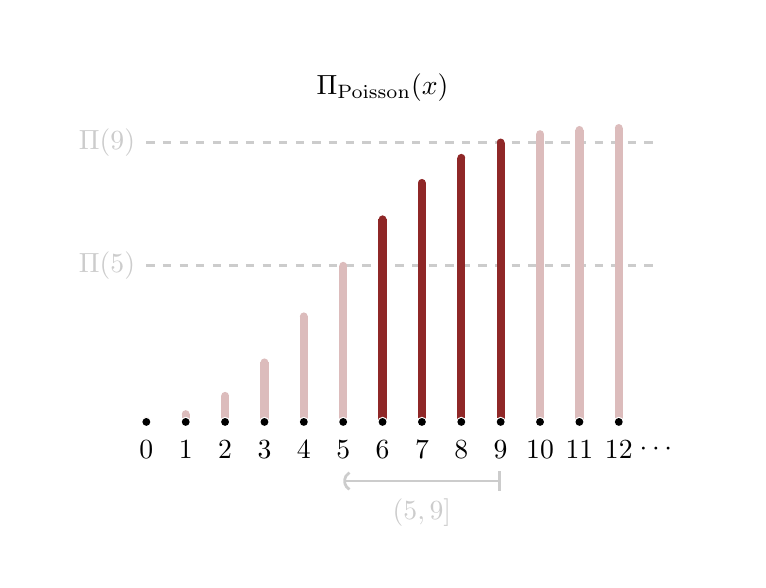
\begin{tikzpicture}[scale=1]
  \begin{scope}[shift={(10, 0)}]
    \draw[white] (-4.5, -3.75) rectangle (4.5, 3);
    
    \draw[gray80, dashed, line width=1] (-3, {3.75 * 0.528919 - 2}) -- (3.5, {3.75 * 0.528919 - 2});
    \node[gray80] at (-3.5, {3.75 * 0.528919 - 2}) { $\Pi(5)$ };
    
    \draw[gray80, dashed, line width=1] (-3, {3.75 * 0.946223 - 2}) -- (3.5, {3.75 * 0.946223 - 2});
    \node[gray80] at (-3.5, {3.75 * 0.946223 - 2}) { $\Pi(9)$ };
    
    \foreach [count=\n] \m in {0.004087, 0.026564, 0.088376, 0.201699, 0.357518, 0.528919, 0.686036, 0.809485, 0.894357, 0.946223, 0.974749, 0.989012, 0.995549} {
      \pgfmathsetmacro{\x}{0.5 * ( (\n - 1) - 6)};
      \draw[light, line width=3] (\x, -2) -- (\x, {(3.75 * \m - 2)});
      \fill[light] (\x, {(3.75 * \m - 2)}) circle (0.05);
      \fill[white] (\x, -2) circle (0.065);
      \fill[black] (\x, -2) circle (0.05);
      
      \pgfmathtruncatemacro{\nn}{\n - 1}
      \node at (\x, -2.35) { $\nn$ };
    }
    
    \foreach [count=\n] \m in {0.686036, 0.809485, 0.894357, 0.946223} {
      \pgfmathsetmacro{\x}{0.5 * ( (\n - 1 + 6) - 6)};
      \draw[dark, line width=3] (\x, -2) -- (\x, {(3.75 * \m - 2)});
      \fill[dark] (\x, {(3.75 * \m - 2)}) circle (0.05);
      \fill[white] (\x, -2) circle (0.065);
      \fill[black] (\x, -2) circle (0.05);
    }
 
    \node at (3.5, -2.35) { $\cdots$ };
 
    \pgfmathsetmacro{\xa}{0.5 * (5 - 6)};
    \pgfmathsetmacro{\xb}{0.5 * (9 - 6)};
    \draw[gray80, arrows={Parenthesis[sharp]-|}, line width=1] (\xa, -2.75) -- (\xb, -2.75);
    \node[gray80] at ({0.5 * (\xa + \xb)}, -3.15) { $(5, 9]$ };
    
    \node at (0, 2.25) { $\Pi_{\mathrm{Poisson}}(x)$ };
  \end{scope}
  
\end{tikzpicture}

\end{document}  